\documentclass[a4paper,12pt]{scrartcl}

\usepackage[utf8]{inputenc} 
\usepackage[T1]{fontenc}
\usepackage[english]{babel}
\usepackage{amsmath, amssymb,amsfonts}
\usepackage{graphicx}
\usepackage{csquotes}
\usepackage{geometry}
\usepackage{float}
\usepackage{framed, xcolor} 
\usepackage{scrlayer-scrpage}
\usepackage{siunitx}
\usepackage{subcaption}
\usepackage{chemgreek}
\usepackage{chemformula}
\usepackage[bookmarks,colorlinks=true]{hyperref}
\usepackage{booktabs}

% 1. ZUERST DIE VARIABLEN DEFINIEREN
\newcommand{\VERSUCHSDATUM}{March 6, 2026}
\newcommand{\PROTOKOLLDATUM}{\today}
\newcommand{\VerfasserEINS}{Julian Brügger}
\newcommand{\MatNoEINS}{3715444}
\newcommand{\EmailEINS}{st190050@stud.uni-stuttgart.de}
\newcommand{\StudiengangEINS}{B.Sc. Chemie}
\newcommand{\VerfasserZWEI}{Benedict Roßkopf}
\newcommand{\MatNoZWEI}{3718292}
\newcommand{\EmailZWEI}{st188124@stud.uni-stuttgart.de}
\newcommand{\StudiengangZWEI}{B.Sc. Simulation Technology}
\newcommand{\BETREUER}{}
\newcommand{\GRUPPENNR}{Gruppe X} % Darf nicht leer sein, wenn im Header genutzt
\newcommand{\VERSUCHSNR}{1}
\newcommand{\VERSUCHSNAME}{Koopmans’ Theorem and Canonical Orbitals}

% 2. DANN DAS LAYOUT
\geometry{left = 2.5cm, top = 3cm}
\renewcaptionname{english}{\figurename}{Fig.}
\renewcaptionname{english}{\tablename}{Tab.}

\sisetup{
    detect-weight=true, 
    detect-family=true,
    locale=UK,
    exponent-product = \cdot,
    separate-uncertainty=true,
    per-mode = symbol-or-fraction
}

\DeclareSIUnit{\angstrom}{\text{\AA}}

\hypersetup{
    colorlinks,
    linktocpage,
    citecolor=black,
    filecolor=black,
    linkcolor=black,
    urlcolor=black
}

\setlength{\parindent}{0 mm}
\setlength{\parskip}{2 mm} 

\pagestyle{scrheadings}
\clearpairofpagestyles % Löscht alte Voreinstellungen
\ihead{\VERSUCHSNR} 
\ofoot{\thepage} 

\begin{document}

\begin{titlepage}
\begin{center}
\Huge{\textbf{\VERSUCHSNAME}}\\
\vspace{10mm}
\Large{Protocol for the Computational Chemistry course by \\ \textbf{\VerfasserEINS\;\& \VerfasserZWEI }}\\
\vspace{10mm} 
\Large{University of Stuttgart}\\
\end{center}
\begin{center}
\begin{tabular}{ll}
\large{authors:}        & \large{\VerfasserEINS, \MatNoEINS} \\
                        & \large{\EmailEINS} \\
                        \vspace{2mm}\\
                        & \large{\VerfasserZWEI, \MatNoZWEI} \\
                        & \large{\EmailZWEI} \\						
                        \vspace{0cm}\\
\large{date of experiment:}	& \large{\VERSUCHSDATUM} \\
\vspace{0cm}\\
\large{submission date:} & \large{\PROTOKOLLDATUM}
\end{tabular}
\end{center}
\end{titlepage}

\section{Introduction}

The Hartree-Fock (HF) method provides the standard computational framework for determining canonical molecular orbitals, which are eigenfunctions of the Fock operator. These orbitals are typically delocalized over the entire molecular framework, reflecting global electronic properties rather than localized bonds. 

A central application of these canonical orbitals is Koopmans' theorem, which approximates the ionization potential ($IP_n$) of a molecule as the negative of the corresponding orbital energy ($\epsilon_n$):

\begin{equation}
IP_{n} = E_{n}^{+} - E \approx -\epsilon_{n}
\end{equation}

This theorem relies on the "frozen orbital approximation," assuming that the remaining orbitals do not relax or rearrange when an electron is removed. While computationally efficient—requiring only a single calculation of the neutral species—it neglects orbital relaxation and electron correlation effects. 

To account for these deficiencies, the $\Delta SCF$ method is used, where the ionization energy is calculated as the direct difference between the converged energies of the neutral molecule ($E$) and its cation ($E_{n}^{+}$):

\begin{equation}
\Delta SCF = E_{n}^{+} - E
\end{equation}

While $\Delta SCF$ allows for orbital relaxation, it can be numerically difficult to converge when the Aufbau principle is not fulfilled. Furthermore, while canonical orbitals are necessary for Koopmans' theorem, they can be transformed into localized orbitals (e.g., via Pipek-Mezey or Boys) to better align with chemical intuition regarding bonds and lone pairs. However, Koopmans' theorem is strictly invalid for such localized representations.

\section{Results and Discussion}

\subsection{Koopmans’ Theorem}

The accuracy of Koopmans' theorem is primarily limited by two competing effects. First, the neglect of orbital relaxation assumes a frozen electron distribution during ionization. This ignores the stabilizing rearrangement of the remaining electrons in the cation, which typically leads to an overestimation of the ionization energy. Second, the neglect of electron correlation in the Hartree-Fock method affects the neutral system more significantly than the cation. Since correlation effects lower the total energy, their omission results in an underestimation of the ionization potential. In many cases, these two errors partially cancel each other out, which explains the surprisingly good agreement with experimental data, particularly for valence orbitals.

The calculated electron affinities (EAs) usually compare less favorably with experimental results than ionization potentials (IPs). This is because the addition of an electron to a neutral molecule significantly increases the electron-electron repulsion. In a Hartree-Fock framework, the virtual orbitals used to describe the EA are often poorly defined as they do not feel the same effective potential as the occupied orbitals. Furthermore, for the negative ion, the effects of electron correlation and orbital relaxation do not cancel out as effectively as they do for cations, leading to larger systematic errors.

The ionization energy calculated via Koopmans' theorem for the HOMO generally agrees better with experimental data than for the energetically lowest core orbitals. For valence electrons, the error caused by the neglect of orbital relaxation is relatively small and is often significantly canceled out by the omission of electron correlation effects. In contrast, removing a core electron creates a highly unstable hole state that leads to a massive rearrangement of all remaining electrons. This large orbital relaxation energy in the core region is no longer effectively compensated by correlation errors, leading to much larger deviations from experimental results for deep-lying levels.

The calculated ionization energies of the canonical orbitals, are displayed in \autoref{tab:n2_ion_results}, together with the experimental values.

\begin{table}[H]
\centering
\caption{\ch{N2} ionization energy values calculated using HF/cc-pVDZ compared to experimental results.}
\label{tab:n2_ion_results}
\begin{tabular}{llcc}
\hline
Orbital & Irrep. & Koopmans' Theorem [eV] & Experiment [eV] \\ \hline
$1\sigma_{g}$    & $A_{g}$         & 426.68                          & 409.80                   \\
$1\sigma_{u}$    & $B_{1u}$        & 426.57                          & 409.80                   \\
$2\sigma_{g}$    & $A_{g}$         & 40.45                           & 37.28                    \\
$2\sigma_{u}$    & $B_{1u}$        & 20.88                           & 18.61                    \\
$1\pi_{u}$       & $B_{2u}$        & 16.79                           & 16.79                    \\
$1\pi_{u}$       & $B_{3u}$        & 16.79                           & 16.79                    \\
$3\sigma_{g}$    & $A_{g}$         & 17.09                           & 15.51                    \\ \hline
\end{tabular}
\end{table}

As observed in the results, the deviation between computed and experimental values is significantly larger for core orbitals. This discrepancy is primarily due to orbital relaxation effects, which are much more pronounced for core electrons than for valence electrons.

The ionization energy of the HOMO was calculated to be \SI{16.80}{\electronvolt} (\SI{0.617}{Hartree}) using Koopmans' theorem, whereas the energy difference method ($\Delta$SCF) yielded a value of \SI{15.91}{\electronvolt} (\SI{0.585}{Hartree}). This discrepancy arises because Koopmans' theorem assumes frozen orbitals, neglecting the orbital relaxation effects of the resulting cation. The $\Delta$SCF method accounts for this relaxation, typically leading to a lower and more accurate ionization potential.

\subsection{Canonical and Localized Orbitals}

The core orbitals shown in \autoref{fig:core} are highly localized at the atomic nuclei and exhibit the highest binding energies. Due to their minimal overlap with neighboring atoms, they do not participate in chemical bonding and remain virtually identical in both the canonical and localized representations.

\begin{figure}[H]
    \centering
    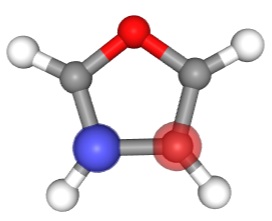
\includegraphics[width=0.5\linewidth]{core.png}
    \caption{Core orbitals of furan localized at the carbon and oxygen nuclei.}
    \label{fig:core}
\end{figure}


In furan, canonical and localized orbitals offer different perspectives on the electronic structure. For $\sigma$-bonds, the localized representation in \autoref{fig:sigma_loc} is more intuitive as it aligns with the Lewis picture of discrete electron pairs and two-center bonds. In contrast, the canonical $\sigma$-orbitals shown in \autoref{fig:sigma_can} are delocalized over the entire molecule, making them harder to interpret chemically. 



\begin{figure}[H]
    \centering
    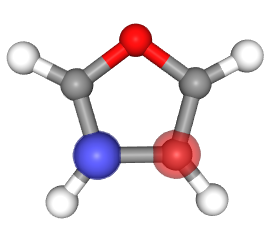
\includegraphics[width=0.5\linewidth]{sigma_loc.png}
    \caption{Localized $\sigma$-orbitals in furan representing discrete bonds.}
    \label{fig:sigma_loc}
\end{figure}

\begin{figure}[H]
    \centering
    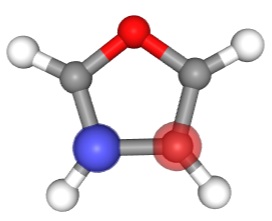
\includegraphics[width=0.5\linewidth]{sigma.png}
    \caption{Canonical $\sigma$-orbitals in furan showing delocalization over the framework.}
    \label{fig:sigma_can}
\end{figure}



For the $\pi$-system, the canonical orbitals in \autoref{fig:pi_can} accurately describe the aromatic delocalization. The localized $\pi$-orbitals in \autoref{fig:pi_loc} artificially break this symmetry into discrete regions, which contradicts the physical nature of the conjugated system.

\begin{figure}[H]
    \centering
    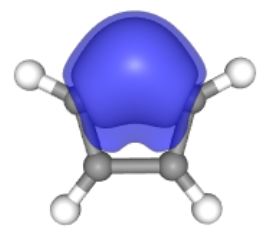
\includegraphics[width=0.5\linewidth]{pi.png}
    \caption{Canonical $\pi$-orbitals illustrating the aromatic system.}
    \label{fig:pi_can}
\end{figure}



\begin{figure}[H]
    \centering
    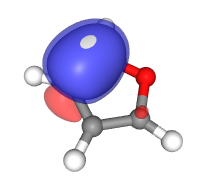
\includegraphics[width=0.5\linewidth]{pi_loc.png}
    \caption{Localized $\pi$-orbitals in furan.}
    \label{fig:pi_loc}
\end{figure}




Koopmans' theorem cannot be applied to localized orbitals because they are not eigenfunctions of the Fock operator. The theorem relates ionization potentials to the eigenvalues of the diagonalized Fock matrix, which are only provided by canonical orbitals. Since localized orbitals are generated through unitary transformations that produce off-diagonal elements, they do not possess a single, physically defined orbital energy.

\section{Conclusion}

The investigation of $N_2$ demonstrates that Koopmans' theorem provides a computationally efficient estimate for ionization potentials, despite neglecting orbital relaxation and electron correlation. The surprisingly good agreement with experimental data for valence orbitals is attributed to a partial cancellation of these two opposing error sources. However, for core orbitals, the lack of relaxation leads to significantly larger deviations. 

The analysis of furan illustrates that while canonical orbitals are the mathematically required basis for Koopmans' theorem, localized orbitals often align better with classical chemical intuition for $\sigma$-bonds and core electrons. In contrast, the delocalized nature of aromatic $\pi$-systems is physically more accurately represented by canonical orbitals. Ultimately, the choice between these representations depends on whether the focus lies on energetic predictions or a qualitative description of chemical bonding.

\end{document}